% Options for packages loaded elsewhere
\PassOptionsToPackage{unicode}{hyperref}
\PassOptionsToPackage{hyphens}{url}
\PassOptionsToPackage{dvipsnames,svgnames,x11names}{xcolor}
%
\documentclass[
]{article}
\usepackage{amsmath,amssymb}
\usepackage{iftex}
\ifPDFTeX
  \usepackage[T1]{fontenc}
  \usepackage[utf8]{inputenc}
  \usepackage{textcomp} % provide euro and other symbols
\else % if luatex or xetex
  \usepackage{unicode-math} % this also loads fontspec
  \defaultfontfeatures{Scale=MatchLowercase}
  \defaultfontfeatures[\rmfamily]{Ligatures=TeX,Scale=1}
\fi
\usepackage{lmodern}
\ifPDFTeX\else
  % xetex/luatex font selection
    \setmainfont[]{NanumGothic}
    \setmonofont[]{UnShinmun}
\fi
% Use upquote if available, for straight quotes in verbatim environments
\IfFileExists{upquote.sty}{\usepackage{upquote}}{}
\IfFileExists{microtype.sty}{% use microtype if available
  \usepackage[]{microtype}
  \UseMicrotypeSet[protrusion]{basicmath} % disable protrusion for tt fonts
}{}
\makeatletter
\@ifundefined{KOMAClassName}{% if non-KOMA class
  \IfFileExists{parskip.sty}{%
    \usepackage{parskip}
  }{% else
    \setlength{\parindent}{0pt}
    \setlength{\parskip}{6pt plus 2pt minus 1pt}}
}{% if KOMA class
  \KOMAoptions{parskip=half}}
\makeatother
\usepackage{xcolor}
\usepackage[margin=1in]{geometry}
\usepackage{color}
\usepackage{fancyvrb}
\newcommand{\VerbBar}{|}
\newcommand{\VERB}{\Verb[commandchars=\\\{\}]}
\DefineVerbatimEnvironment{Highlighting}{Verbatim}{commandchars=\\\{\}}
% Add ',fontsize=\small' for more characters per line
\usepackage{framed}
\definecolor{shadecolor}{RGB}{248,248,248}
\newenvironment{Shaded}{\begin{snugshade}}{\end{snugshade}}
\newcommand{\AlertTok}[1]{\textcolor[rgb]{0.94,0.16,0.16}{#1}}
\newcommand{\AnnotationTok}[1]{\textcolor[rgb]{0.56,0.35,0.01}{\textbf{\textit{#1}}}}
\newcommand{\AttributeTok}[1]{\textcolor[rgb]{0.13,0.29,0.53}{#1}}
\newcommand{\BaseNTok}[1]{\textcolor[rgb]{0.00,0.00,0.81}{#1}}
\newcommand{\BuiltInTok}[1]{#1}
\newcommand{\CharTok}[1]{\textcolor[rgb]{0.31,0.60,0.02}{#1}}
\newcommand{\CommentTok}[1]{\textcolor[rgb]{0.56,0.35,0.01}{\textit{#1}}}
\newcommand{\CommentVarTok}[1]{\textcolor[rgb]{0.56,0.35,0.01}{\textbf{\textit{#1}}}}
\newcommand{\ConstantTok}[1]{\textcolor[rgb]{0.56,0.35,0.01}{#1}}
\newcommand{\ControlFlowTok}[1]{\textcolor[rgb]{0.13,0.29,0.53}{\textbf{#1}}}
\newcommand{\DataTypeTok}[1]{\textcolor[rgb]{0.13,0.29,0.53}{#1}}
\newcommand{\DecValTok}[1]{\textcolor[rgb]{0.00,0.00,0.81}{#1}}
\newcommand{\DocumentationTok}[1]{\textcolor[rgb]{0.56,0.35,0.01}{\textbf{\textit{#1}}}}
\newcommand{\ErrorTok}[1]{\textcolor[rgb]{0.64,0.00,0.00}{\textbf{#1}}}
\newcommand{\ExtensionTok}[1]{#1}
\newcommand{\FloatTok}[1]{\textcolor[rgb]{0.00,0.00,0.81}{#1}}
\newcommand{\FunctionTok}[1]{\textcolor[rgb]{0.13,0.29,0.53}{\textbf{#1}}}
\newcommand{\ImportTok}[1]{#1}
\newcommand{\InformationTok}[1]{\textcolor[rgb]{0.56,0.35,0.01}{\textbf{\textit{#1}}}}
\newcommand{\KeywordTok}[1]{\textcolor[rgb]{0.13,0.29,0.53}{\textbf{#1}}}
\newcommand{\NormalTok}[1]{#1}
\newcommand{\OperatorTok}[1]{\textcolor[rgb]{0.81,0.36,0.00}{\textbf{#1}}}
\newcommand{\OtherTok}[1]{\textcolor[rgb]{0.56,0.35,0.01}{#1}}
\newcommand{\PreprocessorTok}[1]{\textcolor[rgb]{0.56,0.35,0.01}{\textit{#1}}}
\newcommand{\RegionMarkerTok}[1]{#1}
\newcommand{\SpecialCharTok}[1]{\textcolor[rgb]{0.81,0.36,0.00}{\textbf{#1}}}
\newcommand{\SpecialStringTok}[1]{\textcolor[rgb]{0.31,0.60,0.02}{#1}}
\newcommand{\StringTok}[1]{\textcolor[rgb]{0.31,0.60,0.02}{#1}}
\newcommand{\VariableTok}[1]{\textcolor[rgb]{0.00,0.00,0.00}{#1}}
\newcommand{\VerbatimStringTok}[1]{\textcolor[rgb]{0.31,0.60,0.02}{#1}}
\newcommand{\WarningTok}[1]{\textcolor[rgb]{0.56,0.35,0.01}{\textbf{\textit{#1}}}}
\usepackage{graphicx}
\makeatletter
\def\maxwidth{\ifdim\Gin@nat@width>\linewidth\linewidth\else\Gin@nat@width\fi}
\def\maxheight{\ifdim\Gin@nat@height>\textheight\textheight\else\Gin@nat@height\fi}
\makeatother
% Scale images if necessary, so that they will not overflow the page
% margins by default, and it is still possible to overwrite the defaults
% using explicit options in \includegraphics[width, height, ...]{}
\setkeys{Gin}{width=\maxwidth,height=\maxheight,keepaspectratio}
% Set default figure placement to htbp
\makeatletter
\def\fps@figure{htbp}
\makeatother
\setlength{\emergencystretch}{3em} % prevent overfull lines
\providecommand{\tightlist}{%
  \setlength{\itemsep}{0pt}\setlength{\parskip}{0pt}}
\setcounter{secnumdepth}{-\maxdimen} % remove section numbering
\usepackage{fvextra}
\fvset{breaklines}
\ifLuaTeX
  \usepackage{selnolig}  % disable illegal ligatures
\fi
\usepackage{bookmark}
\IfFileExists{xurl.sty}{\usepackage{xurl}}{} % add URL line breaks if available
\urlstyle{same}
\hypersetup{
  pdftitle={Timeseries\_Analysis\_HW3},
  pdfauthor={Na SeungChan},
  colorlinks=true,
  linkcolor={Maroon},
  filecolor={Maroon},
  citecolor={Blue},
  urlcolor={blue},
  pdfcreator={LaTeX via pandoc}}

\title{Timeseries\_Analysis\_HW3}
\author{Na SeungChan}
\date{2025-04-25}

\begin{document}
\maketitle

\begin{center}\rule{0.5\linewidth}{0.5pt}\end{center}

\section{06}\label{section}

\begin{Shaded}
\begin{Highlighting}[]
\FunctionTok{set.seed}\NormalTok{(}\DecValTok{1}\NormalTok{)}
\NormalTok{phi }\OtherTok{\textless{}{-}} \FunctionTok{runif}\NormalTok{(}\DecValTok{1}\NormalTok{, }\SpecialCharTok{{-}}\DecValTok{1}\NormalTok{, }\DecValTok{1}\NormalTok{)}
\NormalTok{theta }\OtherTok{\textless{}{-}} \FunctionTok{runif}\NormalTok{(}\DecValTok{1}\NormalTok{, }\SpecialCharTok{{-}}\DecValTok{1}\NormalTok{, }\DecValTok{1}\NormalTok{)}
\FunctionTok{set.seed}\NormalTok{(}\DecValTok{1}\NormalTok{)}
\NormalTok{Xt }\OtherTok{\textless{}{-}} \FunctionTok{arima.sim}\NormalTok{(}\AttributeTok{n =} \DecValTok{100}\NormalTok{, }\AttributeTok{model =} \FunctionTok{list}\NormalTok{(}\AttributeTok{ar =}\NormalTok{ phi, }\AttributeTok{ma =}\NormalTok{ theta))}
\NormalTok{Xt}
\end{Highlighting}
\end{Shaded}

\begin{verbatim}
## Time Series:
## Start = 1 
## End = 100 
## Frequency = 1 
##   [1]  1.86592877 -0.87188639 -0.31204424 -1.90947290  2.58685499 -1.54582734
##   [7]  0.72026784  0.61018377  0.29366739  0.24614727  0.65164699  0.24149467
##  [13] -0.23872491 -1.89646401  2.01801558 -1.16106488  0.40307885 -1.61994434
##  [19]  0.65772393  0.23176836  1.14309473 -0.98636464  0.87654772 -0.56403860
##  [25] -1.09877447  0.45249764 -0.50036773  0.27619092  0.98566615  0.01958149
##  [31] -0.36889085 -0.03828099  0.77971430  0.01274078 -0.83709874 -0.13875957
##  [37]  0.61060124  0.38892888 -0.49130111  1.14025222 -0.36199790 -0.54407211
##  [43]  0.75280718 -1.56965873  2.45800355  0.46113986 -1.08997971 -0.43903533
##  [49]  1.04265932 -0.76975081  2.79715806 -1.96527770  1.62145627 -0.90883510
##  [55] -0.32420691  0.53093348 -2.10224128  2.91309174 -1.58775510  2.87804642
##  [61] -1.42989459 -0.16096325  0.86778569 -1.49726869 -0.31254280  0.75864289
##  [67] -0.87362026  0.52419099 -0.17177786 -0.52797306 -0.17028724  0.09012143
##  [73]  1.17039384 -2.37375957  2.09685386 -0.80234080  1.35423098 -1.21118491
##  [79]  1.01583926 -0.30394534 -0.46828603  1.56623653  0.11694997  0.34859062
##  [85]  1.24426931 -0.43089047 -1.21734618  0.32414012 -1.23001482  0.41665237
##  [91] -0.69469617  0.52657648 -1.16864812  0.93907471 -1.13541062  2.46718664
##  [97] -0.89234792  1.14537043 -0.38575259  1.76483111
\end{verbatim}

\section{07}\label{section-1}

\subsection{난수 생성}\label{uxb09cuxc218-uxc0dduxc131}

\begin{Shaded}
\begin{Highlighting}[]
\NormalTok{phis }\OtherTok{\textless{}{-}} \FunctionTok{c}\NormalTok{()}

\FunctionTok{set.seed}\NormalTok{(}\DecValTok{1}\NormalTok{)}
\ControlFlowTok{for}\NormalTok{ (i }\ControlFlowTok{in} \DecValTok{1}\SpecialCharTok{:}\DecValTok{500}\NormalTok{) \{}
  \CommentTok{\# time{-}series data generation}
\NormalTok{  Xt }\OtherTok{\textless{}{-}} \FunctionTok{arima.sim}\NormalTok{(}\AttributeTok{n =} \DecValTok{100}\NormalTok{, }\AttributeTok{model =} \FunctionTok{list}\NormalTok{(}\AttributeTok{ar =} \FloatTok{0.5}\NormalTok{))}
  
  \CommentTok{\# saving LSE}
\NormalTok{  phi\_hat }\OtherTok{\textless{}{-}} \FunctionTok{as.numeric}\NormalTok{(}\FunctionTok{lm}\NormalTok{(}\AttributeTok{formula =}\NormalTok{ Xt[}\SpecialCharTok{{-}}\FunctionTok{length}\NormalTok{(Xt)] }\SpecialCharTok{\textasciitilde{}}\NormalTok{ Xt[}\SpecialCharTok{{-}}\DecValTok{1}\NormalTok{] }\SpecialCharTok{+} \DecValTok{0}\NormalTok{)}\SpecialCharTok{$}\NormalTok{coef)}
\NormalTok{  phis }\OtherTok{\textless{}{-}} \FunctionTok{append}\NormalTok{(phis, phi\_hat)}
\NormalTok{\}}

\FunctionTok{head}\NormalTok{(phis)}
\end{Highlighting}
\end{Shaded}

\begin{verbatim}
## [1] 0.5187736 0.4342065 0.3910718 0.5330833 0.4705040 0.4030723
\end{verbatim}

\subsection{히스토그램}\label{uxd788uxc2a4uxd1a0uxadf8uxb7a8}

\begin{Shaded}
\begin{Highlighting}[]
\NormalTok{modified\_data }\OtherTok{\textless{}{-}} \DecValTok{10}\SpecialCharTok{*}\NormalTok{(phis }\SpecialCharTok{{-}} \FloatTok{0.5}\NormalTok{)}

\FunctionTok{hist}\NormalTok{(modified\_data)}
\end{Highlighting}
\end{Shaded}

\begin{center}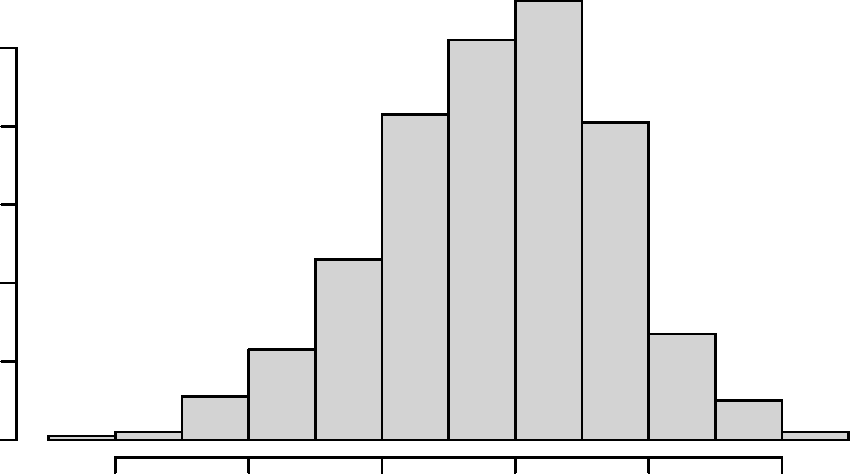
\includegraphics[width=0.8\linewidth]{Timeseries_Analysis_HW3_files/figure-latex/unnamed-chunk-3-1} \end{center}

\subsection{이론적 값과
비교}\label{uxc774uxb860uxc801-uxac12uxacfc-uxbe44uxad50}

\begin{Shaded}
\begin{Highlighting}[]
\FunctionTok{mean}\NormalTok{(modified\_data)}
\end{Highlighting}
\end{Shaded}

\begin{verbatim}
## [1] -0.1416625
\end{verbatim}

\begin{Shaded}
\begin{Highlighting}[]
\FunctionTok{var}\NormalTok{(modified\_data)}
\end{Highlighting}
\end{Shaded}

\begin{verbatim}
## [1] 0.7773941
\end{verbatim}

\begin{Shaded}
\begin{Highlighting}[]
\CommentTok{\# 이론적 값}
\DecValTok{0}
\end{Highlighting}
\end{Shaded}

\begin{verbatim}
## [1] 0
\end{verbatim}

\begin{Shaded}
\begin{Highlighting}[]
\FloatTok{0.75}
\end{Highlighting}
\end{Shaded}

\begin{verbatim}
## [1] 0.75
\end{verbatim}

\(\sigma^2 = 1\)이다. \(E(X_1^2)= \frac{4}{3}\)이다. 즉 이론적 분산은
0.75, 이론적 평균은 0이다.

\begin{Shaded}
\begin{Highlighting}[]
\FunctionTok{set.seed}\NormalTok{(}\DecValTok{1}\NormalTok{)}
\NormalTok{Xt }\OtherTok{\textless{}{-}} \FunctionTok{arima.sim}\NormalTok{(}\AttributeTok{model =} \FunctionTok{list}\NormalTok{(}\AttributeTok{order =} \FunctionTok{c}\NormalTok{(}\DecValTok{1}\NormalTok{,}\DecValTok{0}\NormalTok{,}\DecValTok{0}\NormalTok{), }\AttributeTok{ar =} \FloatTok{0.5}\NormalTok{), }\AttributeTok{n =} \DecValTok{100}\NormalTok{)}
\NormalTok{Xt}
\end{Highlighting}
\end{Shaded}

\begin{verbatim}
## Time Series:
## Start = 1 
## End = 100 
## Frequency = 1 
##   [1]  1.614242003  1.196964238 -0.022758462 -2.226079118  0.011891359
##   [6] -0.038987929 -0.035684228  0.925994097  1.284218243  1.236010443
##  [11]  1.536982593  1.550627597  0.849878782 -1.564412305 -0.162380405
##  [16] -0.137318942 -0.224454978 -1.582979873 -1.269639991 -0.216878436
##  [21]  1.250240334  0.522332440  0.648837831  0.270613875 -1.241752619
##  [26] -1.035870873 -0.912225390 -0.515426092  0.842312326  1.184331911
##  [31]  0.427642359 -0.039540500  0.677193125  0.895259761 -0.241125814
##  [36] -0.828058064 -0.049447070  0.743809390  0.259558483  1.010886968
##  [41]  0.903549364 -0.160251711  0.260993836 -0.998866178  0.933590613
##  [46]  2.447195205  0.856376126 -0.615946563  0.261746346 -0.004181431
##  [51]  2.399527045  1.160523520  1.270001122  0.663002720 -0.411771849
##  [56] -0.017093625 -1.813505441  0.558802141  0.432654409  2.388938875
##  [61]  1.669978966  0.125043052  0.673247880 -0.597473692 -1.552370246
##  [66] -0.484738888 -0.685661317 -0.341725307 -0.096521329 -0.637781611
##  [71] -0.887559538 -0.578958384  0.888607804 -1.079262898  0.054314739
##  [76]  0.360107740  1.243153708  0.317392930  0.528715275  0.531456428
##  [81] -0.276791817  1.069471898  1.695138564  1.547782932  2.360724920
##  [86]  1.738848886 -0.407167766 -0.776849297 -1.613037263 -1.279919268
##  [91] -1.260326311 -0.588047283 -1.204945290 -0.444443872 -0.876806580
##  [96]  1.328883979  1.381149466  1.600748962  1.184559839  2.274456000
\end{verbatim}

\subsection{LSE 계산}\label{lse-uxacc4uxc0b0}

\begin{Shaded}
\begin{Highlighting}[]
\FunctionTok{as.numeric}\NormalTok{(}\FunctionTok{lm}\NormalTok{(}\AttributeTok{formula =}\NormalTok{ Xt[}\SpecialCharTok{{-}}\FunctionTok{length}\NormalTok{(Xt)] }\SpecialCharTok{\textasciitilde{}}\NormalTok{ Xt[}\SpecialCharTok{{-}}\DecValTok{1}\NormalTok{] }\SpecialCharTok{+} \DecValTok{0}\NormalTok{)}\SpecialCharTok{$}\NormalTok{coef)}
\end{Highlighting}
\end{Shaded}

\begin{verbatim}
## [1] 0.5187736
\end{verbatim}

\section{09}\label{section-2}

\subsection{데이터 입력}\label{uxb370uxc774uxd130-uxc785uxb825}

\begin{Shaded}
\begin{Highlighting}[]
\NormalTok{Xt }\OtherTok{\textless{}{-}} \FunctionTok{read.csv}\NormalTok{(}\StringTok{\textquotesingle{}ex\_ch3\_8.txt\textquotesingle{}}\NormalTok{, }\AttributeTok{sep =} \StringTok{\textquotesingle{}}\SpecialCharTok{\textbackslash{}n}\StringTok{\textquotesingle{}}\NormalTok{)}
\NormalTok{Xt }\OtherTok{\textless{}{-}} \FunctionTok{ts}\NormalTok{(}\FunctionTok{as.vector}\NormalTok{(Xt)}\SpecialCharTok{$}\NormalTok{data)}
\NormalTok{Xt}
\end{Highlighting}
\end{Shaded}

\begin{verbatim}
## Time Series:
## Start = 1 
## End = 14 
## Frequency = 1 
##  [1]  72  71  59  44  74  78  81  64  86  87 104  88  84  62
\end{verbatim}

\href{http://www.freeaca.com/new/library/BoardTableList.aspx}{자유아카데미
홈페이지 자료실}에서 다운로드할 수 있는 `시계열 분석 이론 및 SAS 실습
2판' 교재의 데이터 파일을 내려받아 활용하였다. 파일명이 교재와 다른데,
3장에서 파일을 활용하는 문제가 하나뿐이어서 이름이 3.8 문제에 대응하는
것으로 되어 있는 파일을 활용하였다.

\subsection{CSS
사용(최소제곱추정량)}\label{css-uxc0acuxc6a9uxcd5cuxc18cuxc81cuxacf1uxcd94uxc815uxb7c9}

\begin{Shaded}
\begin{Highlighting}[]
\NormalTok{Xt\_LSE }\OtherTok{\textless{}{-}} \FunctionTok{arima}\NormalTok{(}\AttributeTok{x =}\NormalTok{ Xt, }\AttributeTok{order =} \FunctionTok{c}\NormalTok{(}\DecValTok{1}\NormalTok{, }\DecValTok{0}\NormalTok{, }\DecValTok{1}\NormalTok{), }\AttributeTok{method =} \StringTok{\textquotesingle{}CSS\textquotesingle{}}\NormalTok{)}
\FunctionTok{summary}\NormalTok{(Xt\_LSE)}
\end{Highlighting}
\end{Shaded}

\begin{verbatim}
##           Length Class  Mode     
## coef       3     -none- numeric  
## sigma2     1     -none- numeric  
## var.coef   9     -none- numeric  
## mask       3     -none- logical  
## loglik     1     -none- numeric  
## aic        1     -none- logical  
## arma       7     -none- numeric  
## residuals 14     ts     numeric  
## call       4     -none- call     
## series     1     -none- character
## code       1     -none- numeric  
## n.cond     1     -none- numeric  
## nobs       1     -none- numeric  
## model     10     -none- list
\end{verbatim}

\(\hat{\phi}_{LSE} = 0.4405\)

\(\hat{\theta}_{LSE} = 0.0347\)

\(\hat{\mu}_{LSE} = 74.8414\)

\subsection{ML
사용(최대가능도추정량)}\label{ml-uxc0acuxc6a9uxcd5cuxb300uxac00uxb2a5uxb3c4uxcd94uxc815uxb7c9}

\begin{Shaded}
\begin{Highlighting}[]
\NormalTok{Xt\_MLE }\OtherTok{\textless{}{-}} \FunctionTok{arima}\NormalTok{(}\AttributeTok{x =}\NormalTok{ Xt, }\AttributeTok{order =} \FunctionTok{c}\NormalTok{(}\DecValTok{1}\NormalTok{, }\DecValTok{0}\NormalTok{, }\DecValTok{1}\NormalTok{), }\AttributeTok{method =} \StringTok{\textquotesingle{}ML\textquotesingle{}}\NormalTok{)}
\FunctionTok{summary}\NormalTok{(Xt\_MLE)}
\end{Highlighting}
\end{Shaded}

\begin{verbatim}
##           Length Class  Mode     
## coef       3     -none- numeric  
## sigma2     1     -none- numeric  
## var.coef   9     -none- numeric  
## mask       3     -none- logical  
## loglik     1     -none- numeric  
## aic        1     -none- numeric  
## arma       7     -none- numeric  
## residuals 14     ts     numeric  
## call       4     -none- call     
## series     1     -none- character
## code       1     -none- numeric  
## n.cond     1     -none- numeric  
## nobs       1     -none- numeric  
## model     10     -none- list
\end{verbatim}

\(\hat{\phi}_{MLE} = 0.4109\)

\(\hat{\theta}_{MLE} = 0.0342\)

\(\hat{\mu}_{MLE} = 74.4687\)

\end{document}
